\section{Introduction to an app store}
\label{sec:introduction_to_an_app_store}

A software platform is comprised of the technology that makes up the platform as well as the human beings that use the technology. Over time, a platform has to evolve, under go changes, support more developers and reach out to more users of the platform. Most software platforms use app stores to support the growth process. \cite{Jansen} describes an app store as ``An online curated market-place that allows developers to sell and distribute their products to actors within one or more multi-sided software platform ecosystems.''

He describes that an app store system as one that should:

\begin{enumerate}
  \item be available using the internet,
  \item be curated by an organization, typically but not necessarily the platform owner,
  \item allow for the selling and buying of software products,
  \item take care of the financial transactions involved in selling the software products,
  \item have two distinct user groups: \emph{developers} and \emph{users},
  \item be serving one or more software ecosystem, and
  \item implement a platform that takes care of the distribution of the software products.
\end{enumerate}

\begin{figure}
  \centering
  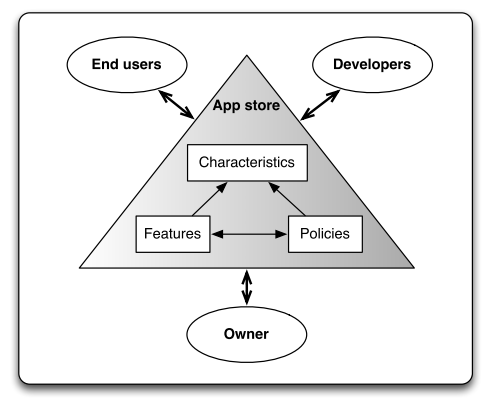
\includegraphics[width=9cm]{figures/app_store_triangle.png}
  \caption{Conceptual Model of an app store. (Source~\cite{Jansen})}
  \label{fig:conceptual_model_of_app_store}
\end{figure}

According to \cite{Jansen}, to create a better understanding of app store within the software ecosystem, a conceptual model is created as shown in Figure \ref{fig:conceptual_model_of_app_store}. The ovals show the actors involved in the ecosystem. The first one in the bottom is the owner of the app store. The second oval represents users, those who download and uses the apps. The third oval represents the developers who contributes and places their applications on the repository. They all interact with the triangle. The triangle represents the app store. The rectangles inside the triangle describe the processes inside the app store. The first rectangle represents Policies which act as guidelines for users and developers. The second rectangle represent Features. Both policies and features can be influenced by platform owner. The third rectangle represents the characteristics which cannot be directly influenced by the platform owner like the number of developers, number of users, quality of apps or the usability of the app store. However an owner can modify the policies and the features to influence the characteristics of the app store.

Features and policies complement eachother. Features make an app store have more interesting ways for users to interact with. At the same time, the guidelines defined by Policies prevent the app store from being misused. Enforcing Policies are even harder than defining them. Big companies like Google and Apple have plenty of technical and human resources to check the quality of apps in their app stores. In smaller ecosystems, these resources are not readily available. Non the less, certain features can be introduced that makes enforcing policies easier. \cite{Jansen} studied six different mobile app stores: Google's PlayStore, Apple's App Store, SlideMe, Binpress, Amazon app store and Intel AppUp. They listed 69 characteristic features of a typical app store under 12 different categories. We list 6 features below that play part in convergence process.

\begin{itemize}
  \item \textbf{Recommendations} offer users new software based on their existing profile.
  \item \textbf{App categories} segregate Apps into distinct groups based on their features.
  \item \textbf{App lists} (e.g. top lists, latest additions) allow users to discover popular and new softwares.
  \item \textbf{Search} allow users to find the software by using plain text words.
  \item \textbf{Ratings} provide a feedback mechanism to other users know about the quality of software.
  \item \textbf{Review} are text comments describing users opinion of the software.
\end{itemize}

\section*{Conclusion}

App stores play a central role in a software platform. S2Store is the app store for pervasive computing platform DS2OS. It consists of features that allow developers to share context models and services. S2Store allows users to find and use uploaded services and provide feedback about their quality using S2Store's features. The analysis done in \cite{Jansen} is a good reference point for S2Store's feature sets.

